\section{Kružnice a řezy}
\subsection{Řez}\label{rez}
Ať $G$ je \hyperref[souvisly]{souvislý} graf. Množina hran $S \subseteq E$ je \ii{řez}, jestliže existuje rozklad $V$ na dvě neprázdné množiny $V_1, V_2$ takové, že
\begin{equation}
	S = \bc{e \mid e = \bc{u,v}, u \in V_1, v \in V_2}.
\end{equation}
$S$ značíme $\langle V_1, V_2\rangle$.

Příklady řezů v grafu
\begin{figure}[H]
    \centering
    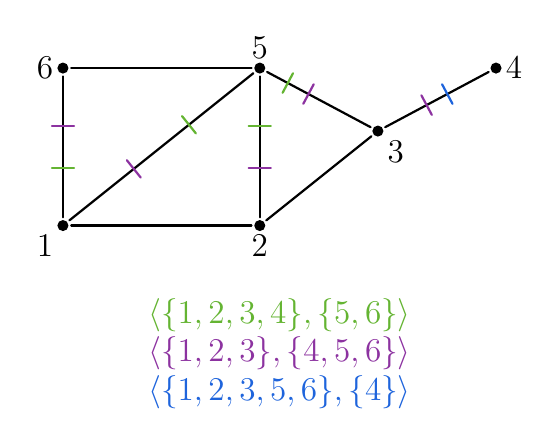
\begin{tikzpicture}[
        scale=1,
        vertex/.style={circle, fill=black, minimum size=4pt, inner sep=0pt, outer sep=1pt},
        label_node/.style={font=\large},
        edge/.style={thick, draw=black, line cap=round},
        cut mark/.style={thick, line cap=round}
    ]

        \definecolor{mygreen}{RGB}{100, 180, 50}
        \definecolor{mypurple}{RGB}{140, 50, 160}
        \definecolor{myblue}{RGB}{30, 100, 220}

        \node[vertex] (v1) at (0, 0) {};
        \node[label_node, below left] at (v1) {1};

        \node[vertex] (v2) at (2.5, 0) {};
        \node[label_node, below] at (v2) {2};

        \node[vertex] (v3) at (4, 1.2) {};
        \node[label_node, below right] at (v3) {3};

        \node[vertex] (v4) at (5.5, 2) {};
        \node[label_node, right] at (v4) {4};

        \node[vertex] (v5) at (2.5, 2) {};
        \node[label_node, above] at (v5) {5};

        \node[vertex] (v6) at (0, 2) {};
        \node[label_node, left] at (v6) {6};

        \draw[edge] (v1) -- (v2);
        \draw[edge] (v2) -- (v3);
        \draw[edge] (v6) -- (v5);

        \draw[edge] (v1) -- node[pos=0.35, sloped, allow upside down] {\tikz \draw[cut mark, mygreen] (0,-4pt) -- (0,4pt);}
                            node[pos=0.65, sloped, allow upside down] {\tikz \draw[cut mark, mypurple] (0,-4pt) -- (0,4pt);} 
                    (v6);

        \draw[edge] (v1) -- node[pos=0.35, sloped, allow upside down] {\tikz \draw[cut mark, mypurple] (0,-4pt) -- (0,4pt);}
                            node[pos=0.65, sloped, allow upside down] {\tikz \draw[cut mark, mygreen] (0,-4pt) -- (0,4pt);}
                    (v5);

        \draw[edge] (v2) -- node[pos=0.35, sloped, allow upside down] {\tikz \draw[cut mark, mypurple] (0,-4pt) -- (0,4pt);}
                            node[pos=0.65, sloped, allow upside down] {\tikz \draw[cut mark, mygreen] (0,-4pt) -- (0,4pt);}
                    (v5);

        \draw[edge] (v3) -- node[pos=0.6, sloped, allow upside down] {\tikz \draw[cut mark, mypurple] (0,-4pt) -- (0,4pt);}
                            node[pos=0.8, sloped, allow upside down] {\tikz \draw[cut mark, mygreen] (0,-4pt) -- (0,4pt);}
                    (v5);

        \draw[edge] (v3) -- node[pos=0.4, sloped, allow upside down] {\tikz \draw[cut mark, mypurple] (0,-4pt) -- (0,4pt);}
                            node[pos=0.6, sloped, allow upside down] {\tikz \draw[cut mark, myblue] (0,-4pt) -- (0,4pt);}
                    (v4);


        \node[below, align=left, font=\large] at (2.75, -0.8) {
            \textcolor{mygreen}{$\langle \{1,2,3,4\}, \{5,6\} \rangle$} \\
            \textcolor{mypurple}{$\langle \{1,2,3\}, \{4,5,6\} \rangle$} \\
            \textcolor{myblue}{$\langle \{1,2,3,5,6\}, \{4\} \rangle$}
        };
    \end{tikzpicture}
\end{figure}
 
\subsection{Věta o dvou různých řezech}
Jsou dány dva různé \hyperref[rez]{řezy} $S_1 = \langle V_1, V_2 \rangle$, $S_2 = \langle W_1, W_2\rangle$ \hyperref[souvisly]{souvislého} neorientovaného grafu $G$. Pak $S_1 \oplus S_2$ je také řez grafu $G$.

\dukaz
\begin{figure}[H]
    \centering
    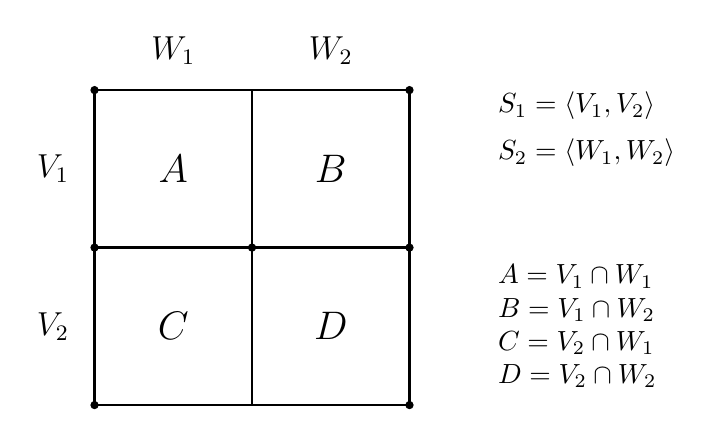
\begin{tikzpicture}[scale=1]
        \tikzset{
            part/.style={font=\Large},
            label_text/.style={font=\large}
        }
        \draw[thick] (0,0) rectangle (4,4);
        
        \draw[thick] (0,2) -- (4,2);
		\draw[thick] (2,0) -- (2,4);
        
        \node[part] at (1,3) {$A$};
        \node[part] at (3,3) {$B$};
        \node[part] at (1,1) {$C$};
        \node[part] at (3,1) {$D$};

        \node[label_text, left] at (-0.2, 3) {$V_1$};
        \node[label_text, left] at (-0.2, 1) {$V_2$};

        \node[label_text, above] at (1, 4.2) {$W_1$};
        \node[label_text, above] at (3, 4.2) {$W_2$};

        \foreach \x in {0,4} \foreach \y in {0,4}
            \fill (\x,\y) circle (1.5pt);
		\fill (0, 2) circle (1.5pt);
        \fill (2, 2) circle (1.5pt);
		\fill (4, 2) circle (1.5pt);
		
        \begin{scope}[xshift=5cm, yshift=2.5cm]
            \node[right, align=left] at (0, 1) {
                $S_1 = \langle V_1, V_2 \rangle$ \\[0.5em]
                $S_2 = \langle W_1, W_2 \rangle$
            };
            \node[right, align=left] at (0, -1.5) {
                $A = V_1 \cap W_1$ \\
                $B = V_1 \cap W_2$ \\
                $C = V_2 \cap W_1$ \\
                $D = V_2 \cap W_2$
            };
        \end{scope}
    \end{tikzpicture}
\end{figure}
A víme
\begin{align}
A \cup B &\not= \emptyset \\
A \cup C &\not= \emptyset \\
B \cup D &\not= \emptyset \\
C \cup D &\not= \emptyset
\end{align}
Označme: $X, Y \in \bc{A,B,C,D}$. $[X,Y] = \bc{e = \bc{u,v} \mid u \in X, v \in Y}$.
\begin{equation}
	\langle V_1, V_2\rangle = [A, C] \cup [A, D] \cup [B, C] \cup [B, D]
\end{equation}
A protože jsou disjunktní, namísto $\cup$ můžeme psát $\oplus$.
\begin{equation}
	\langle W_1, W_2\rangle = [A, B] \oplus [A, D] \oplus [C, B] \oplus [C, D]
\end{equation}
\begin{align}
	\langle V_1, V_2\rangle \oplus \langle W_1, W_2 \rangle &= [A, B] \oplus [A, C] \oplus [B, D] \oplus [C, D] \\
	\langle V_1, V_2\rangle \oplus \langle W_1, W_2 \rangle &= \langle A \cup D, B \cup C\rangle
\end{align}
Ověřme $A \cup D \not= \emptyset \not= B \cup C$. To by muselo platit $V_1 = W_2$ a $V_2 = W_1$, což neplatí.
\hspace{\fill}\qed

\subsection{Prostor řezů}\label{prostorRezu}
Je dán \hyperref[souvisly]{souvislý} graf $G = (V, E)$. \ii{Prostor řezů} je vektorový podprostor generovaný množinou všech \hyperref[rez]{řezů} grafu $G$. Značíme ho $(W_R, \oplus, \emptyset, \cdot)$.

\ii{Jinými slovy $W_R = \bc{S \mid S \text{ je řez}} \cup \bc{\emptyset}$}.

\subsection{Cutset}\label{cutset}
Je dán \hyperref[souvisly]{souvislý} graf $G = (V, E)$. \ii{Cutset} (min-řez) je minimální (ne nejmenší, ale minimální) množina $S \subseteq E$ taková, že $G \setminus S$ je nesouvislý graf.
% TODO: nákresy

\subsection{Tvrzení o souvislosti cutsetů}
Je dán \hyperref[rez]{řez} $S = \langle V_1, V_2 \rangle$ souvislého neorientovaného grafu $G$. Pak $S$ je \hyperref[cutset]{cutsetem} právě tehdy, když podgrafy indukované množinami $V_1$ a $V_2$ jsou \hyperref[souvisly]{souvislé}.
% TODO: nákres

\subsection{Tvrzení o řezu a kostrách}
Množina hran $S \subseteq E$ je \hyperref[rez]{řez} právě tehdy, když má s každou kostrou $T$ grafu $G$ neprázdný průnik, tj. $S \cap T \not= \emptyset$.

\dukaz\\
\enquote{$\Rightarrow$}: $S \subseteq E$ je řez. Tzn. $G \setminus S$ je \hyperref[souvisly]{nesouvislý}. Mějme libovolnou kostru $T$. Kdyby $T \cap S = \emptyset$, tak v $G \setminus S$ existují hrany $T$. Tj. $G \setminus S$ je souvislý. Což je spor.

\enquote{$\Leftarrow$}: Předpokládejme, že $T \cap S \not= \emptyset \, \forall T$.\\
Kdyby $G \setminus S$ bylo souvislé, tak existuje kostra $T_1$ grafu $G \setminus S$. Vrcholy jsou stejné, takže $T_1$ je kostra $G$. To ale znamená $S \cap T_1 = \emptyset$. Takže $G \setminus S$ musí být nesouvislé. Což je spor.
\hspace{\fill}\qed

\subsection{Prostor kružnic}\label{prostorKruznic}
Je dán \hyperref[souvisly]{souvislý} graf $G=(V, E)$. \ii{Prostor kružnic} je vektorový prostor generovaný množinou všech \hyperref[kruznice]{kružnic} grafu $G$. Značíme ho $(W_K, \oplus, \emptyset, \cdot)$.

\subsection{Věta o prostoru kružnic a sudých stupních}
Podmnožina $K \subseteq E$ patří do \hyperref[prostorKruznic]{prostoru kružnic} $W_K$ právě tehdy, když v grafu $(V, K)$ má každý vrchol sudý stupeň.

\dukaz\\
\enquote{$\Rightarrow$}: Podmnožina $K \subseteq E$ patří do prostoru kružnic $W_K$. Ukažme, že pokud $A, B$ splňují podmínku sudosti stupňů, tj. každý vrchol má sudý stupeň, tak $A \oplus B$ také splňuje podmínku.
\begin{equation}
	A \oplus B = (A \cup B)\setminus(A \cap B)
\end{equation}
Vyberme libovolný vrchol $v \in V$. Spočítejme $d_{A \oplus B}(v)$. Hrany, které zbydou v $A \oplus B$ jsou hrany $(A^\prime \setminus B^\prime) \cup  B^\prime \setminus A^\prime)=K_v$.
\begin{align}
	|K_v^\prime| = |(A^\prime \cup B^\prime) \setminus (A^\prime \cap B^\prime)| = ((|A^\prime| +  B^\prime|) - |A^\prime \cap B^\prime| - |A^\prime \cap B^\prime|) = \underbrace{|A^\prime|}_{d_A(v)} + \underbrace{|B^\prime|}_{d_B(v)} - 2\underbrace{|A^\prime \cap B^\prime|}_{l}
\end{align}
Máme tedy
\begin{equation}
	d_{A \oplus B}(v) = d_A(v) + d_B(v) - 2,
\end{equation}
kde $l$ je počet hran incidentních s $v$, které leží jak v $A$, tak v $B$, tedy opět sudé číslo. Rozdíl sudých čísel je také sudé číslo.

\enquote{$\Leftarrow$}: Předpokládejme, že množina hran $A$ splňuje podmínku sudosti stupňů; tj. $d_A(v)$ je sudé pro každý vrchol $v \in V$.

Jestliže každý vrchol $v$ má v $A$ nulový stupeň, pak $A = \emptyset$ a $A$ leží v prostoru kružnic $W_K$; ano, $\emptyset=0 \cdot K$ pro libovolnou kružnici $K$.

Předpokládejme, že některý vrchol $v$ má stupeň větší než 0. Pak $d_A(v) \geq 2$. Generujme náhodně tah z vrcholu $v$. Protože každý vrchol, do kterého se dostaneme má vždy ještě alespoň jednu nepoužitou hranu, jednou se vrátíme do vrcholu, ve kterém tah již byl. Tím jsme uzavřeli kružnici, označme ji $K_1$. Vytvoříme $A \oplus K_1 = A \setminus K_1$. Protože každý vrchol měl v kružnici $K_1$ sudý stupeň, má sudý stupeň i v $A \setminus K_1$. Nyní buď $A_1 = A \setminus K_1$ je prázdná množina, nebo postup opakujeme pro množinu $A \setminus K_1$. Po konečně mnoha krocích dostaneme kružnice $K_1, K_2, \dots, K_l$ takové, že
\begin{equation}
	(\dots (A \setminus K_1) \dots K_l) = \emptyset, \, \text{proto } A = K_1 \cup \dots \cup K_l = K_1 \oplus \dots \oplus K_l.
\end{equation}
Tedy $A \in W_K$.
\hspace{\fill}\qed 
